\documentclass[12pt]{article}
\usepackage[utf8]{inputenc}
\usepackage{graphicx}
\usepackage{titling}
\usepackage{datetime}
\usepackage{enumitem}
\usepackage{xcolor}
\usepackage{listings}
\usepackage{multirow}

% Título de la tarea
\title{\vspace{1cm}Proyecto Final de Bases de Datos}
\date{} % Deja la fecha en blanco

% Ajustar márgenes para la portada
\usepackage[left=3cm,right=3cm,top=3cm,bottom=3cm]{geometry}

% Comando para agregar los escudos
\newcommand{\doubleshield}[2]{%
    \begin{minipage}[t]{0.48\textwidth}
        \centering
        \includegraphics[width=0.5\linewidth]{#1}
        \par\vspace{1ex}
        %Escudo #1
    \end{minipage}\hfill%
    \begin{minipage}[t]{0.48\textwidth}
        \centering
        \includegraphics[width=0.5\linewidth]{#2}
        \par\vspace{1ex}
        %Escudo #2
    \end{minipage}%
}

\begin{document}

\lstset{
    language=SQL,                   % Lenguaje de programación
    basicstyle=\ttfamily,              % Fuente y estilo básico
    keywordstyle=\color{red},         % Estilo de las palabras clave
    commentstyle=\color{green},        % Estilo de los comentarios
    numbers=left,                      % Números de línea a la izquierda
    numberstyle=\tiny\color{gray},     % Estilo de los números de línea
    frame=single,                      % Borde alrededor del código
    breaklines=true,                   % Romper líneas largas
    postbreak=\mbox{\textcolor{red}{$\hookrightarrow$}\space}, % Flecha de ruptura de línea
    showstringspaces=false             % No mostrar espacios en cadenas
}


\pagecolor{black}
\color{white}

\begin{titlepage}
    \begin{center}
        \vspace*{2cm}
        
        % Agrega los escudos aquí
        \doubleshield{UNAM.png}{EFC.png}
        
        \vspace{2cm}
        
        \Huge{\thetitle}
        
        \vspace{4cm}
        
        \Large{Tarea presentada por:}
        
        \vspace{0.5cm}
        
        \Large{Edgar Montiel Ledesma 317317794 \\ Carlos Daniel Cortes Jimenez 420004846}
        
        \vfill
        
        Facultad de Ciencias \\
        Universidad Nacional Autónoma de Méixco \\
        Fecha de Entrega: 11 de Diciembre de 2023 % Cambia la fecha de entrega        
    \end{center}
\end{titlepage}
    
    \section*{Base de Datos: Sistema de Administración de Tienda en Línea}

    \subsection*{1. Lista de Requerimientos}
    % Lista de requerimientos aquí
        \begin{itemize}
            \item[1.] Registro de Clientes:
                \begin{itemize}
                    \item La base de datos debe permitir el registro de nuevos clientes, incluyendo su nombre, dirección y número de teléfono.
                \end{itemize}
            \item[2.] Registro de Autos:
                \begin{itemize}
                    \item La base de datos debe permitir el registro de nuevos autos, incluyendo información como modelo, marca, año de fabricación y precio.
                \end{itemize}
            \item[3.] Registro de Empleados:
                \begin{itemize}
                    \item La base de datos debe permitir el registro de empleados, especificando su nombre, dirección, número de teléfono y rol en la agencia (gerente, asesor, promotor, mecánico, electromecánico, etc.).
                \end{itemize}
            \item[4.] Registro de Servicios:
                \begin{itemize}
                    \item La base de datos debe permitir el registro de servicios ofrecidos por la agencia, incluyendo nombre del servicio, descripción y precio.
                \end{itemize}
            \item[5.] Registro de Mantenimientos:
                \begin{itemize}
                    \item La base de datos debe permitir el registro de mantenimientos realizados, especificando el auto involucrado, el cliente, el empleado a cargo, el servicio proporcionado y la fecha del mantenimiento.
                \end{itemize}
            \item[6.] Registro de Trabajos de Hojalatería y Pintura:
                \begin{itemize}
                    \item La base de datos debe permitir el registro de trabajos de hojalatería y pintura, indicando el auto, el cliente, el empleado responsable, el servicio proporcionado y la fecha del trabajo.
                \end{itemize}
            \item[7.] Registro de Seguros para Autos:
                \begin{itemize}
                    \item La base de datos debe permitir el registro de seguros para autos, detallando el auto asegurado, el cliente, el tipo de seguro, la cobertura y el precio del seguro.
                \end{itemize}
            \item[8.] Relaciones entre Entidades:
                \begin{itemize}
                    \item La base de datos debe establecer y mantener relaciones adecuadas entre las entidades, como la asociación de autos con clientes, empleados con mantenimientos y servicios con mantenimientos.
                \end{itemize}
            \item[9.] Consulta de Información:
                \begin{itemize}
                    \item Debe ser posible realizar consultas para obtener información detallada, como el historial de mantenimientos de un auto, los clientes asociados a un empleado.
                \end{itemize}
            \item[10.] Integridad Referencial:
                \begin{itemize}
                    \item La base de datos debe garantizar la integridad referencial, asegurando que las claves foráneas estén correctamente vinculadas a las claves primarias correspondientes.
                \end{itemize}
            \item[11.] Manejo de Precios en Decimal:
                \begin{itemize}
                    \item Los precios deben manejarse con precisión decimal, considerando los campos que almacenan valores monetarios.
                \end{itemize}
            \item[12.] Registro de Fechas:
                \begin{itemize}
                    \item La base de datos debe almacenar fechas de manera precisa para rastrear la temporalidad de eventos como mantenimientos, trabajos de hojalatería y pintura.
                \end{itemize}
        \end{itemize}

    \subsection*{2. Modelo Conceptual (Notación de Peter Chen)}
    \begin{figure}[h]
        \centering
        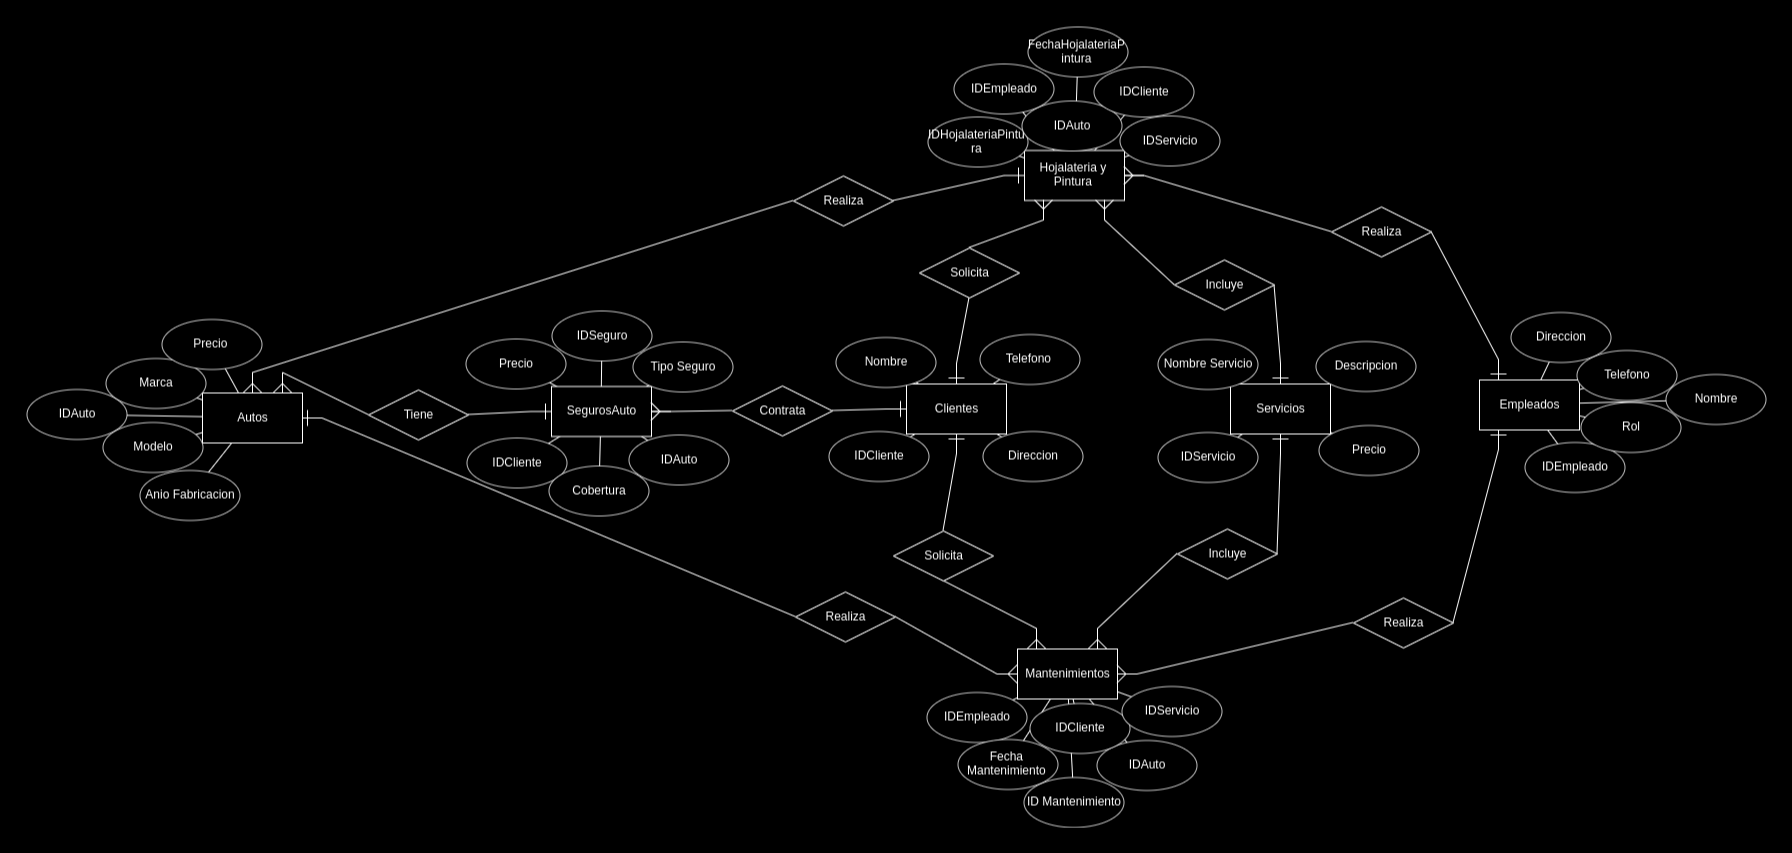
\includegraphics[width=0.9\textwidth]{EAuto.png}
        \caption{Modelo Conceptual}
        \label{fig:modelo-conceptual}
    \end{figure}

    \subsection*{3. Modelo Relacional}
    \begin{figure}[h]
        \centering
        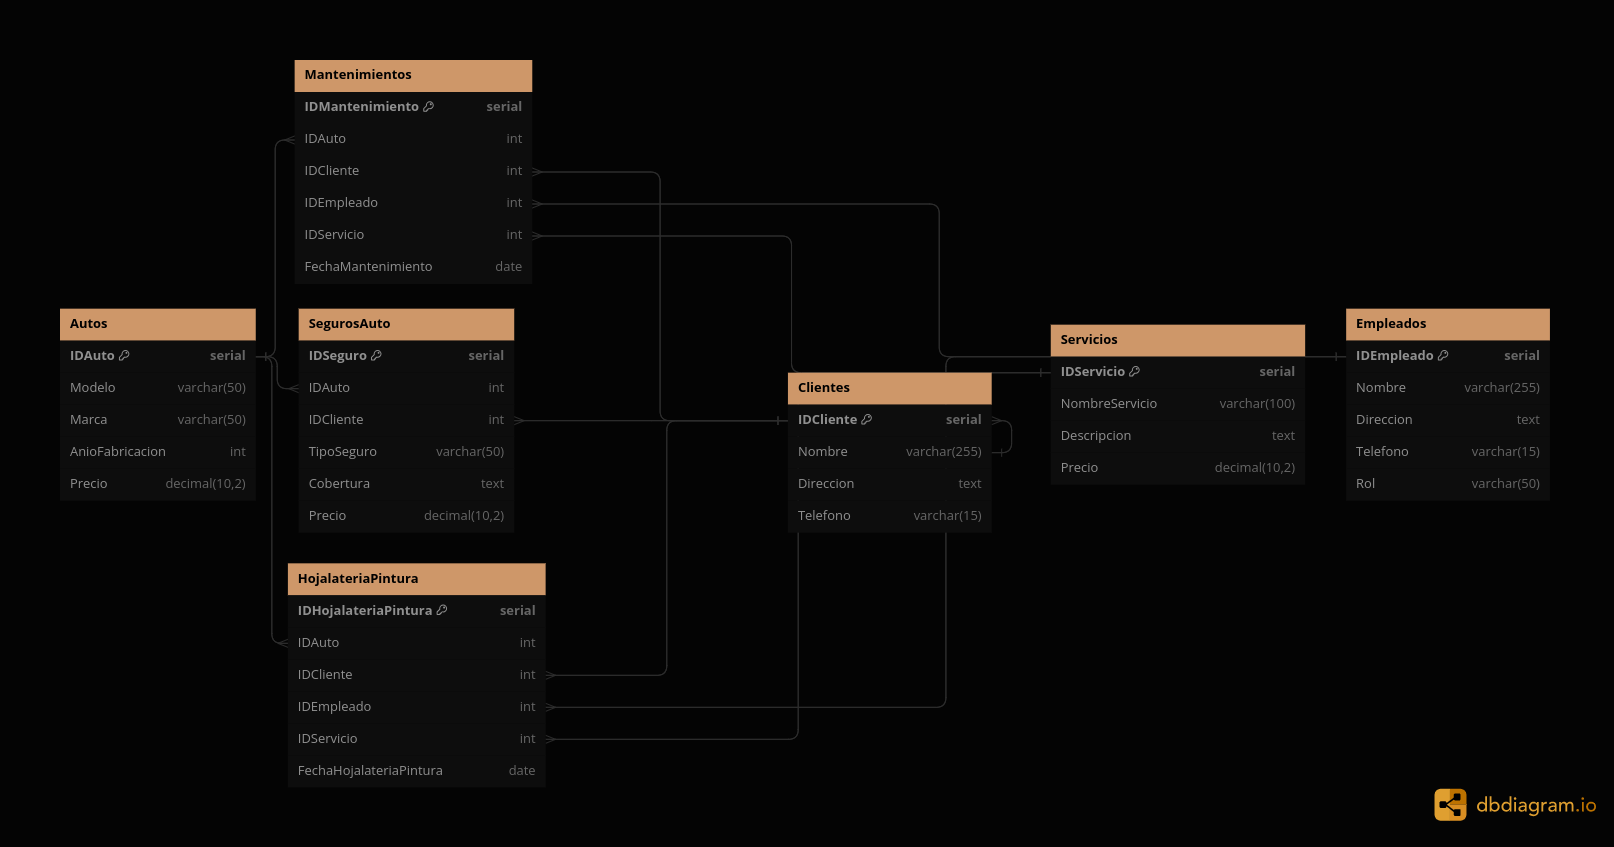
\includegraphics[width=1.0\textwidth]{ERAuto.png}
        \caption{Modelo Conceptual}
        \label{fig:modelo-conceptual}
    \end{figure}

    \subsection*{4. Script Completo para Crear la Base de Datos}
    \begin{lstlisting}[language=SQL]
CREATE TABLE "Clientes" (
  "IDCliente" serial PRIMARY KEY,
  "Nombre" varchar(255),
  "Direccion" text,
  "Telefono" varchar(15)
);

CREATE TABLE "Autos" (
  "IDAuto" serial PRIMARY KEY,
  "Modelo" varchar(50),
  "Marca" varchar(50),
  "AnioFabricacion" int,
  "Precio" decimal(10,2)
);

CREATE TABLE "Empleados" (
  "IDEmpleado" serial PRIMARY KEY,
  "Nombre" varchar(255),
  "Direccion" text,
  "Telefono" varchar(15),
  "Rol" varchar(50)
);

CREATE TABLE "Servicios" (
  "IDServicio" serial PRIMARY KEY,
  "NombreServicio" varchar(100),
  "Descripcion" text,
  "Precio" decimal(10,2)
);

CREATE TABLE "Mantenimientos" (
  "IDMantenimiento" serial PRIMARY KEY,
  "IDAuto" int,
  "IDCliente" int,
  "IDEmpleado" int,
  "IDServicio" int,
  "FechaMantenimiento" date
);

CREATE TABLE "HojalateriaPintura" (
  "IDHojalateriaPintura" serial PRIMARY KEY,
  "IDAuto" int,
  "IDCliente" int,
  "IDEmpleado" int,
  "IDServicio" int,
  "FechaHojalateriaPintura" date
);

CREATE TABLE "SegurosAuto" (
  "IDSeguro" serial PRIMARY KEY,
  "IDAuto" int,
  "IDCliente" int,
  "TipoSeguro" varchar(50),
  "Cobertura" text,
  "Precio" decimal(10,2)
);
    \end{lstlisting}

    \subsection*{5. Script de Inserción de Datos (para 100 registros)}
    \begin{lstlisting}[language=SQL]
-- Script de Inserción de Datos para las tablas 
-- Inserción de Datos para la Tabla Clientes
INSERT INTO Clientes (Nombre, Direccion, Telefono) VALUES
('Juan Pérez', 'Calle 123, Ciudad A', '555-1234'),
('Maria Rodriguez', 'Avenida XYZ, Ciudad B', '555-5678'),
('Carlos Martinez', 'Calle 456, Ciudad C', '555-9876'),
('Laura Lopez', 'Avenida LMN, Ciudad A', '555-5432'),
('Pedro Sanchez', 'Calle 789, Ciudad B', '555-8765'),
('Ana Gutierrez', 'Avenida PQR, Ciudad C', '555-2345'),
('Javier Hernandez', 'Calle 012, Ciudad A', '555-6789'),
('Sofia Ramirez', 'Avenida DEF, Ciudad B', '555-3456'),
('Alejandro Torres', 'Calle 345, Ciudad C', '555-8765'),
('Isabel Castro', 'Avenida UVW, Ciudad A', '555-2345'),
('Luis Morales', 'Calle 678, Ciudad B', '555-7890'),
('Elena Navarro', 'Avenida GHI, Ciudad C', '555-4567'),
('Raul Jimenez', 'Calle 901, Ciudad A', '555-0987'),
('Carmen Ortega', 'Avenida JKL, Ciudad B', '555-6543'),
('Ricardo Vargas', 'Calle 234, Ciudad C', '555-5678'),
('Patricia Diaz', 'Avenida STU, Ciudad A', '555-4321'),
('Daniel Mendoza', 'Calle 567, Ciudad B', '555-8765'),
('Monica Silva', 'Avenida NOP, Ciudad C', '555-3210'),
('Roberto Cruz', 'Calle 890, Ciudad A', '555-7654'),
('Martha Flores', 'Avenida ABC, Ciudad B', '555-2109'),
('Gabriel Vega', 'Calle 123, Ciudad C', '555-6543'),
('Veronica Herrera', 'Avenida XYZ, Ciudad A', '555-0987'),
('Hector Nuñez', 'Calle 456, Ciudad B', '555-5432'),
('Silvia Torres', 'Avenida LMN, Ciudad C', '555-8765'),
('Juan Ramírez', 'Calle 123, Ciudad B', '123-456-7890'),
('Maria Rodriguez', 'Avenida YZ, Ciudad H', '977-654-3210'),
('Carlos López', 'Carrera 456, Ciudad C', '456-789-0123'),
('Ana Martinez', 'Avenida ABC, Ciudad A', '789-012-3456'),
('Pedro Sánchez', 'Calle 789, Ciudad B', '012-345-6789'),
('Laura González', 'Carrera 789, Ciudad C', '345-678-9012'),
('Roberto Jiménez', 'Calle 456, Ciudad A', '678-901-2345'),
('Sofía Torres', 'Avenida XYZ, Ciudad B', '901-234-5678'),
('Miguel Ruiz', 'Carrera 123, Ciudad C', '234-567-8901'),
('Carmen Herrera', 'Avenida ABC, Ciudad A', '567-890-1234'),
('Diego Flores', 'Calle 789, Ciudad B', '890-123-4567'),
('Isabel Castro', 'Carrera 456, Ciudad C', '123-234-5678'),
('Javier Nuñez', 'Avenida XYZ, Ciudad A', '234-345-6789'),
('Adriana Vega', 'Calle 123, Ciudad B', '345-456-7890'),
('Hector Mendoza', 'Carrera 789, Ciudad C', '456-567-8901'),
('Luisa Ramos', 'Avenida ABC, Ciudad A', '567-678-9012'),
('Oscar Díaz', 'Calle 456, Ciudad B', '678-789-0123'),
('Raquel Silva', 'Avenida XYZ, Ciudad C', '789-890-1234'),
('Fernando Ortiz', 'Carrera 123, Ciudad A', '890-901-2345'),
('Natalia Vargas', 'Calle 789, Ciudad B', '901-012-3456'),
('Eduardo Guzmán', 'Avenida ABC, Ciudad C', '012-123-2345'),
('Gabriela Paredes', 'Carrera 456, Ciudad A', '123-234-3456'),
('Alberto Navarro', 'Avenida XYZ, Ciudad B', '234-345-4567'),
('Marta Jiménez', 'Calle 123, Ciudad C', '345-456-5678'),
('Juan Martínez', 'Calle C #123', '555-1334'),
('María García', 'Avenida B #456', '555-5678'),
('Carlos López', 'Calle C #789', '555-9876'),
('Ana Rodríguez', 'Avenida D #1011', '555-1112'),
('Miguel Sánchez', 'Calle E #1314', '555-1314'),
('Laura Martínez', 'Avenida F #1516', '555-1516'),
('Javier Torres', 'Calle G #1718', '555-1718'),
('Rosa Ramírez', 'Avenida H #1920', '555-1920'),
('Pedro Gómez', 'Calle I #2122', '555-2122'),
('Carmen Vargas', 'Avenida J #2324', '555-2324'),
('Roberto Castro', 'Calle K #2526', '555-2526'),
('Sofía Jiménez', 'Avenida L #2728', '555-2728'),
('Fernando Reyes', 'Calle M #2930', '555-2930'),
('Isabel Herrera', 'Avenida N #3132', '555-3132'),
('Alejandro Medina', 'Calle O #3334', '555-3334'),
('Patricia Torres', 'Avenida P #3536', '555-3536'),
('Luis Soto', 'Calle Q #3738', '555-3738'),
('Elena Navarro', 'Avenida R #3940', '555-3940'),
('Héctor Mendoza', 'Calle S #4142', '555-4142'),
('Marta Guzmán', 'Avenida T #4344', '555-4344'),
('Daniel Herrera', 'Calle U #4546', '555-4546'),
('Beatriz Salazar', 'Avenida V #4748', '555-4748'),
('Ricardo Márquez', 'Calle W #4950', '555-4950'),
('Susana Vidal', 'Avenida X #5152', '555-5152'),
('Jorge Ramos', 'Calle Y #5354', '555-5354'),
('Juan Pérez', 'Calle H #13', '555-1244'),
('María Rodríguez', 'Avenida B #456', '555-5678'),
('Pedro Gómez', 'Calle C #789', '555-9012'),
('Laura Martínez', 'Avenida D #1011', '555-3456'),
('Carlos Sánchez', 'Calle E #1213', '555-7890'),
('Ana López', 'Avenida F #1415', '555-2345'),
('Javier Torres', 'Calle G #1617', '555-6789'),
('Carmen Ramírez', 'Avenida H #1819', '555-0123'),
('Roberto Herrera', 'Calle I #2021', '555-4567'),
('Sofía González', 'Avenida J #2223', '555-8901'),
('Daniel Jiménez', 'Calle K #2425', '555-2345'),
('Isabel Castro', 'Avenida L #2627', '555-6789'),
('Miguel Díaz', 'Calle M #2829', '555-0123'),
('Patricia Vargas', 'Avenida N #3031', '555-4567'),
('Raúl Flores', 'Calle O #3233', '555-8901'),
('Elena Mendoza', 'Avenida P #3435', '555-2345'),
('Luisa Vega', 'Calle Q #3637', '555-6789'),
('Adrián Navarro', 'Avenida R #3839', '555-0123'),
('Beatriz Ortega', 'Calle S #4041', '555-4567'),
('Gabriel Ruiz', 'Avenida T #4243', '555-8901'),
('Monica Salazar', 'Calle U #4445', '555-2345'),
('Héctor Núñez', 'Avenida V #4647', '555-6789'),
('Silvia Paredes', 'Calle W #4849', '555-0123'),
('Alejandro Medina', 'Avenida X #5051', '555-4567'),
('Rosa Soto', 'Calle Y #5253', '555-8901');
('Fernando Alvarez', 'Calle M #2930', '555-2930'),
('Isabel Fernandez', 'Avenida N #3132', '555-3132'),

-- Inserción de Datos para la Tabla Autos
INSERT INTO Autos (Modelo, Marca, AnioFabricacion, Precio) VALUES
('Sedán', 'Toyota', 2020, 25000.00),
('SUV', 'Honda', 2019, 28000.00),
('Coupé', 'Ford', 2021, 32000.00),
('Camioneta', 'Chevrolet', 2022, 35000.00),
('Hatchback', 'Volkswagen', 2018, 20000.00);
('Fusion', 'Ford', 2023, 27000.00),
('Altima', 'Nissan', 2022, 24000.00),
('Cruze', 'Chevrolet', 2021, 21000.00),
('Malibu', 'Chevrolet', 2023, 26000.00),
('Sentra', 'Nissan', 2022, 23000.00),
('Focus', 'Ford', 2021, 20000.00),
('Maxima', 'Nissan', 2023, 29000.00),
('Mustang', 'Ford', 2022, 35000.00),
('Corvette', 'Chevrolet', 2021, 70000.00),
('Rav4', 'Toyota', 2023, 32000.00),
('Camaro', 'Chevrolet', 2022, 40000.00),
('Escape', 'Ford', 2021, 27000.00),
('Pathfinder', 'Nissan', 2023, 31000.00),
('CR-V', 'Honda', 2022, 30000.00),
('Explorer', 'Ford', 2021, 34000.00),
('Armada', 'Nissan', 2023, 38000.00),
('Pilot', 'Honda', 2022, 33000.00),
('Tacoma', 'Toyota', 2021, 32000.00),
('Tundra', 'Toyota', 2023, 36000.00),
('Frontier', 'Nissan', 2022, 29000.00),
('Sedan', 'Toyota', 2022, 25000.00),
('SUV', 'Honda', 2021, 30000.00),
('Compacto', 'Ford', 2020, 20000.00),
('Pickup', 'Chevrolet', 2022, 35000.00),
('Coupe', 'BMW', 2021, 40000.00),
('Familiar', 'Volkswagen', 2020, 28000.00),
('Deportivo', 'Audi', 2022, 45000.00),
('Híbrido', 'Lexus', 2021, 32000.00),
('Crossover', 'Nissan', 2020, 27000.00),
('Camioneta', 'Jeep', 2022, 38000.00),
('Convertible', 'Mercedes-Benz', 2021, 50000.00),
('Subcompacto', 'Hyundai', 2020, 22000.00),
('Camión', 'Ram', 2022, 40000.00),
('SUV Compacto', 'Mazda', 2021, 28000.00),
('Minivan', 'Chrysler', 2020, 32000.00),
('Coupé Deportivo', 'Porsche', 2022, 55000.00),
('Auto Eléctrico', 'Tesla', 2021, 60000.00),
('SUV de Lujo', 'Jaguar', 2020, 70000.00),
('Roadster', 'Ferrari', 2022, 80000.00),
('Berlina', 'Volvo', 2021, 35000.00),
('Microcoche', 'Smart', 2020, 18000.00),
('Monovolumen', 'Kia', 2022, 30000.00),
('Hatchback', 'Subaru', 2021, 24000.00),
('Compacto Deportivo', 'Alfa Romeo', 2020, 38000.00),
('Coupé de Lujo', 'Lamborghini', 2022, 90000.00),
('Sedan', 'Toyota', 2022, 25000.00),
('Hatchback', 'Volkswagen', 2021, 20000.00),
('SUV', 'Honda', 2023, 30000.00),
('Pickup', 'Ford', 2020, 35000.00),
('Coupe', 'Chevrolet', 2022, 28000.00),
('Convertible', 'Mazda', 2021, 32000.00),
('Sedan', 'Hyundai', 2023, 26000.00),
('Hatchback', 'Kia', 2020, 23000.00),
('SUV', 'Nissan', 2022, 27000.00),
('Pickup', 'Ram', 2021, 33000.00),
('Coupe', 'BMW', 2020, 40000.00),
('Convertible', 'Audi', 2023, 38000.00),
('Sedan', 'Mercedes-Benz', 2021, 35000.00),
('Hatchback', 'Ford', 2022, 24000.00),
('SUV', 'Jeep', 2020, 32000.00),
('Pickup', 'Chevrolet', 2023, 37000.00),
('Coupe', 'Lexus', 2021, 29000.00),
('Convertible', 'Tesla', 2022, 45000.00),
('Sedan', 'Subaru', 2023, 26000.00),
('Hatchback', 'Volvo', 2020, 22000.00),
('SUV', 'Mitsubishi', 2021, 28000.00),
('Pickup', 'GMC', 2022, 36000.00),
('Coupe', 'Jaguar', 2020, 42000.00),
('Convertible', 'Porsche', 2023, 50000.00),
('Sedan', 'Acura', 2021, 31000.00);
('Sedán A1', 'Audi', 2022, 35000.00),
('Civic', 'Honda', 2021, 28000.00),
('Camry', 'Toyota', 2022, 32000.00),
('Accord', 'Honda', 2020, 30000.00),
('Mustang', 'Ford', 2021, 42000.00),
('Corolla', 'Toyota', 2023, 27000.00),
('C-Class', 'Mercedes-Benz', 2022, 50000.00),
('Rogue', 'Nissan', 2021, 32000.00),
('X5', 'BMW', 2023, 60000.00),
('Wrangler', 'Jeep', 2022, 35000.00),
('F-150', 'Ford', 2022, 38000.00),
('3 Series', 'BMW', 2021, 42000.00),
('Camaro', 'Chevrolet', 2023, 45000.00),
('Mazda3', 'Mazda', 2022, 26000.00),
('Pilot', 'Honda', 2020, 34000.00),
('Q5', 'Audi', 2023, 48000.00),
('Highlander', 'Toyota', 2021, 36000.00),
('Escalade', 'Cadillac', 2022, 75000.00),
('Grand Cherokee', 'Jeep', 2023, 42000.00),
('GLC', 'Mercedes-Benz', 2021, 52000.00),
('Civic Type R', 'Honda', 2022, 38000.00),
('Charger', 'Dodge', 2021, 41000.00),
('Malibu', 'Chevrolet', 2023, 29000.00),
('Mazda CX-5', 'Mazda', 2022, 31000.00),
('Atlas', 'Volkswagen', 2021, 36000.00);

-- Inserción de Datos para la Tabla Empleados
INSERT INTO Empleados (Nombre, Direccion, Telefono, Rol) VALUES
('Laura Sánchez', 'Calle 456, Ciudad C', '555-1111', 'Asesor'),
('Héctor Nuñez', 'Calle 753, Ciudad XYZ', '555-4545', 'Asesor'),
('Javier García', 'Avenida XYZ, Ciudad B', '555-2222', 'Mecánico'),
('Lucía Vargas', 'Calle 135, Ciudad XYZ', '555-7777', 'Mecánico'),
('Sofía Vargas', 'Carrera 789, Ciudad A', '555-3333', 'Promotor'),
('María González', 'Avenida ABC, Ciudad XYZ', '555-5678', 'Promotor'),
('Raúl Díaz', 'Calle 246, Ciudad XYZ', '555-6666', 'Promotor'),
('Daniel Mendoza', 'Avenida K, Ciudad P', '888888888', 'Promotor'),
('Daniel Ruiz', 'Calle 123, Ciudad A', '555-4444', 'Electromecánico'),
('Laura Gomez', 'Avenida D, Ciudad W', '666666666', 'Electromecánico'),
('Elena Torres', 'Avenida LMN, Ciudad B', '555-5555', 'Gerente');

-- Inserción de Datos para la Tabla Servicios
INSERT INTO Servicios (NombreServicio, Descripcion, Precio) VALUES
('Cambio de Aceite', 'Incluye cambio de aceite y filtro.', 50.00),
('Revisión de Frenos', 'Revisión y ajuste de sistema de frenos.', 80.00),
('Alineación y Balanceo', 'Alineación y balanceo de ruedas.', 60.00),
('Cambio de Batería', 'Sustitución de batería.', 100.00),
('Diagnóstico Electrónico', 'Análisis electrónico del sistema.', 120.00),
('Cambio de Neumáticos', 'Cambio de neumáticos', 200.00),
('Lavado y Encerado', 'Lavado exterior y encerado', 30.00),
('Reparación de Aire Acondicionado', 'Reparación del sistema de aire acondicionado', 150.00),
('Cambio de Correa de Distribución', 'Reemplazo de correa de distribución', 90.00),
('Revisión de Suspensión', 'Inspección y mantenimiento de suspensión', 75.00),
('Cambio de Filtros', 'Cambio de filtros de aire y combustible', 40.00),
('Recarga de Refrigerante', 'Recarga del sistema de refrigeración', 60.00),
('Inspección de Luces', 'Inspección y reemplazo de luces', 20.00),
('Cambio de Pastillas de Freno', 'Reemplazo de pastillas de freno', 70.00),
('Reparación de Escape', 'Reparación de sistema de escape', 80.00),
('Cambio de Amortiguadores', 'Reemplazo de amortiguadores', 120.00),
('Recarga de Aceite para Dirección', 'Recarga de aceite para dirección', 25.00),
('Reparación de Transmisión', 'Reparación de sistema de transmisión', 180.00),
('Cambio de Bujías', 'Reemplazo de bujías', 30.00),
('Ajuste de Motor', 'Ajuste y mantenimiento del motor', 100.00),
('Reparación de Sistema de Dirección', 'Reparación de problemas en el sistema de dirección', 99.99),
('Reemplazo de Correa de Distribución', 'Reemplazo de correa de distribución y ajuste', 129.99),
('Servicio de Inyección de Combustible', 'Mantenimiento y limpieza del sistema de inyección', 69.99),
('Servicio de Frenos ABS', 'Mantenimiento y reparación del sistema de frenos ABS', 109.99),
('Diagnóstico de Problemas', 'Análisis y diagnóstico de problemas mecánicos', 49.99),
('Inspección de Emisiones', 'Inspección de emisiones contaminantes', 50.00),
('Recarga de Aire Acondicionado', 'Recarga de gas refrigerante y revisión del sistema de aire acondicionado', 69.99),
('Cambio de Termostato', 'Reemplazo de termostato', 45.00),
('Inspección de Neumáticos', 'Revisión del estado y presión de los neumáticos', 30.00),
('Reparación de Sistema Eléctrico', 'Reparación de problemas eléctricos', 120.00),
('Servicio de Transmisión', 'Revisión y mantenimiento de la transmisión', 159.99),
('Cambio de Sensor de Oxígeno', 'Reemplazo de sensor de oxígeno', 60.00),
('Servicio de Limpieza de Inyectores', 'Limpieza y mantenimiento de inyectores', 80.00);

-- Inserción de Datos para la Tabla Mantenimientos
INSERT INTO Mantenimientos (IDAuto, IDCliente, IDEmpleado, IDServicio, FechaMantenimiento) VALUES
(1, 1, 2, 3, '2023-01-15'),
(2, 3, 4, 1, '2023-02-20'),
(3, 2, 1, 2, '2023-03-25'),
(4, 4, 5, 4, '2023-04-10'),
(5, 1, 2, 3, '2023-05-30'),
(6, 3, 1, 2, '2023-06-05'),
(7, 2, 2, 1, '2023-07-10'),
(8, 4, 3, 4, '2023-08-15'),
(9, 1, 1, 3, '2023-09-20'),
(10, 3, 2, 2, '2023-10-25'),
(11, 2, 3, 1, '2023-11-30'),
(12, 4, 1, 4, '2023-12-05'),
(13, 1, 2, 3, '2024-01-10'),
(14, 3, 1, 2, '2024-02-15'),
(15, 2, 2, 1, '2024-03-20'),
(16, 4, 3, 4, '2024-04-25'),
(17, 1, 1, 3, '2024-05-30'),
(18, 3, 2, 2, '2024-06-05'),
(19, 2, 3, 1, '2024-07-10'),
(20, 4, 1, 4, '2024-08-15');
(21, 2, 3, 1, '2024-09-02'),
(22, 1, 2, 3, '2024-10-08'),
(23, 3, 1, 2, '2024-11-15'),
(24, 2, 3, 1, '2024-12-20'),
(25, 1, 2, 3, '2025-01-25');
(26, 3, 1, 2, '2023-02-15'),
(27, 2, 3, 1, '2023-03-20'),
(28, 4, 1, 4, '2023-04-25'),
(29, 5, 3, 5, '2023-05-05'),


-- Inserción de Datos para la Tabla HojalateriaPintura
INSERT INTO HojalateriaPintura (IDAuto, IDCliente, IDEmpleado, IDServicio, FechaHojalateriaPintura) VALUES
(1, 1, 2, 3, '2023-01-20'),
(2, 3, 4, 1, '2023-02-25'),
(3, 2, 1, 2, '2023-03-30'),
(4, 4, 5, 4, '2023-04-15'),
(5, 5, 3, 5, '2023-05-10'),
(6, 16, 6, 3, '2023-01-06'),
(7, 17, 7, 30, '2023-01-07'),
(8, 18, 8, 3, '2023-01-08'),
(9, 19, 9, 9, '2023-01-09'),
(10, 10, 10, 10, '2023-01-10'),
(11, 11, 11, 11, '2023-01-11'),
(12, 12, 2, 12, '2023-01-12'),
(13, 13, 2, 33, '2023-01-13'),
(14, 14, 4, 14, '2023-01-14'),
(15, 15, 5, 15, '2023-01-15'),
(16, 16, 6, 16, '2023-01-16'),
(17, 17, 7, 17, '2023-01-17'),
(18, 18, 8, 18, '2023-01-18'),
(19, 19, 9, 19, '2023-01-19'),
(20, 10, 2, 20, '2023-01-20'),
(21, 11, 1, 32, '2023-01-21'),
(22, 12, 2, 32, '2023-01-22'),
(23, 23, 2, 33, '2023-01-23'),
(24, 24, 4, 24, '2023-01-24'),
(25, 15, 5, 25, '2023-01-25');

-- Inserción de Datos para la Tabla SegurosAuto
INSERT INTO SegurosAuto (IDAuto, IDCliente, TipoSeguro, Cobertura, Precio) VALUES
(1, 1, 'Seguro Básico', 'Cobertura limitada', 300.00),
(2, 3, 'Seguro Completo', 'Cobertura amplia', 500.00),
(3, 2, 'Seguro Básico', 'Cobertura limitada', 300.00),
(4, 4, 'Seguro de Responsabilidad', 'Responsabilidad civil', 200.00),
(5, 5, 'Seguro Completo', 'Cobertura amplia', 500.00);
(6, 6, 'Seguro Básico', 'Cobertura limitada', 550.00),
(7, 7, 'Seguro Completo', 'Cobertura total', 820.00),
(8, 8, 'Seguro Terceros', 'Responsabilidad civil', 320.00),
(9, 9, 'Seguro contra Robo', 'Cobertura contra robo', 620.00),
(10, 10, 'Seguro a Todo Riesgo', 'Cobertura amplia', 920.00),
(11, 11, 'Seguro Básico', 'Cobertura limitada', 510.00),
(12, 12, 'Seguro Completo', 'Cobertura total', 830.00),
(13, 13, 'Seguro Terceros', 'Responsabilidad civil', 310.00),
(14, 14, 'Seguro contra Robo', 'Cobertura contra robo', 630.00),
(15, 15, 'Seguro a Todo Riesgo', 'Cobertura amplia', 910.00),
(16, 16, 'Seguro Básico', 'Cobertura limitada', 525.00),
(17, 17, 'Seguro Completo', 'Cobertura total', 840.00),
(18, 18, 'Seguro Terceros', 'Responsabilidad civil', 330.00),
(19, 19, 'Seguro contra Robo', 'Cobertura contra robo', 640.00),
(20, 20, 'Seguro a Todo Riesgo', 'Cobertura amplia', 930.00);
(21, 21, 'Seguro Completo', 'Cobertura amplia con asistencia en carretera', 580.00),
(22, 22, 'Seguro contra Robo', 'Cobertura contra robo y pérdida total', 460.00),
(23, 23, 'Seguro Básico', 'Responsabilidad civil', 330.00),
(24, 24, 'Seguro Completo', 'Cobertura amplia con asistencia en carretera', 600.00),
(25, 25, 'Seguro contra Robo', 'Cobertura contra robo y pérdida total', 480.00);
    \end{lstlisting}    

    \subsection*{6. Evidencia de Restricciones de Integridad Referencial}
    % Incluir evidencias aquí

    \subsection*{7. Evidencia de Restricciones CHECK}
    % Incluir evidencias aquí
    
    \subsection*{8. Evidencia de Dominios Personalizados}
    % Incluir evidencias aquí
    
    \subsection*{9. Evidencia de Restricciones para Tuplas}
    % Incluir evidencias aquí
    
    \subsection*{10. Consultas Relevantes}
    % Consultas aquí
    
    \subsection*{11. Vistas Relevantes}
    % Vistas aquí
\end{document}

